\chapter{Redes Ópticas Elásticas Multicore y Fragmentación del Ancho de Banda}
Las redes ópticas que se basan en WDM dividen el espectro de cada enlace en canales cuyo ancho de banda se fija de 50 GHz o 100 GHz. Esto debido a que la Unión Internacional de Telecomunicaciones (\textit{ITU-T International Telecommunication Union}) especificó el estándar G.694.1 en el año 2002.
%
Estas redes WDM resultan muy rígidas, y debido a eso es posible que ocurra una utilización ineficiente de la capacidad, provocado por el hecho de que el espacio entre dos canales adyacentes es relativamente grande y si la señal que se transmite utiliza un ancho de banda muy bajo, gran parte del espectro será desperdiciado.
%

Una nueva tecnología denominada Redes Ópticas Elásticas o \textit{Elastic Optical Networks} (EON) y su evolución: Las Redes ópticas Elásticas Multinúcleo o \textit{Multicore Elastic Optical Networks} (MC-EON) el cual no solo dividen el espectro óptico en Ranuras de Frecuencia o \textit{Frequency Slots} (FS) de 12.5 GHz conforme a lo establecido por el estándar definido en ITU-T (G.694.1) en el año 2012, sino que las (MC-EON) introducen un nuevo dominio de multiplexación espacial, al permitir la transmisión simultánea de múltiples señales ópticas en diferentes núcleos dentro de una misma fibra.
%
Esta aproximación multidimensional proporciona una mayor escalabilidad, eficiencia en la asignación del espectro y reducción del consumo energético, posicionando a las MC-EON como una de las tecnologías mas prometedoras para la implementación de redes ópticas de ultra alta capacidad en escenarios de próxima generación.
%

% En la Figura \ref{fig:eonwdm}, se muestra una comparación en la asignación de demandas en ambas tecnologías, observándose un mejor aprovechamiento del espectro óptico para el caso de las redes EON, debido a un menor desperdicio de ancho en banda.

% % \begin{figure}
% %     \centering
% %     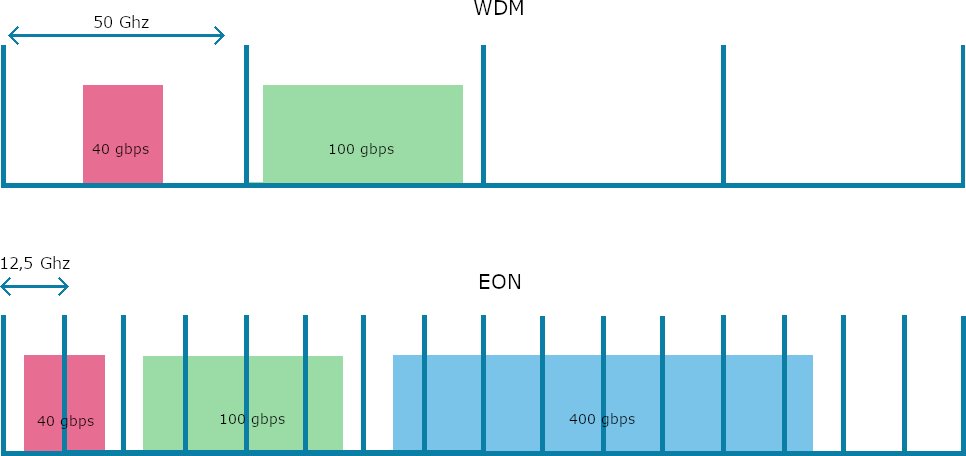
\includegraphics[width=0.95\textwidth]{capitulos/img/eonwdm.png}
% %     \caption{Redes WDM v s Redes EON}
% %     \label{fig:eonwdm}
% % \end{figure}


\section{Fragmentación del Ancho de Banda en EON}
Las redes ópticas elásticas multinúcleo (MC-EON) permiten optimizar el uso del ancho de banda necesario para satisfacer una demanda, respetando tres restricciones fundamentales:
%

\begin{itemize}
    \item \textbf{Restricción de continuidad:} esta restricción implica que un cambio de luz o lightpath debe utilizar los mismos \textit{Frecuency Slots} (FS) a lo largo del camino establecido entre los nodos de origen y destino, tanto en la dimensión espectral como en la dimensión espacial (núcleo).
    \item \textbf{Restricción de consecutividad:} esta restricción establece que todos los FS utilizados para establecer un lightpath deben ser contiguos en el dominio espectral, formando un solo bloque contiguo de FS dentro del mismo núcleo. 
\end{itemize}
%

Estas restricciones conducen a que, tras sucesivas asignaciones y liberaciones de recursos, se genere la aparición de bloques aislados de FS no utilizados tanto en la dimensión espectral como en la dimesión espacial (núcleos) de los enlaces ópticos.
Dichos bloques fragmentados presentan desalineación tanto entre enlaces consecutivos de la ruta como entre los diferentes núcleos de una misma fibra multinúcleo. Como consecuencia, se incrementa significativamente la probabilidad de bloqueo de solicitudes, 
pudiendo la red rechazar demandas incluso cuando existe ancho de banda disponible suficiente en los enlaces. Este fenómeno se denomina \textbf{Fragmentación de la red} y en arquitecturas multinúcleo se manifiesta en dos domensiones complementarias:
%

\begin{itemize}
    \item \textbf{Fragmentación espectral:} se refiere a la presencia de bloques aislados de FS no utilizados en el dominio espectral, que no pueden ser aprovechados para establecer nuevas conexiones debido a las restricciones de continuidad y consecutividad.
    \item \textbf{Fragmentación espacial:} se refiere a la desalineación de bloques de FS disponibles entre los diferentes núcleos de una misma fibra multinúcleo, lo que dificulta la asignación eficiente de recursos en la dimensión espacial.
\end{itemize}
%

\textbf{Ejemplo ilustrativo del fenómeno:}
\begin{enumerate}[1 -]
   \item Se presenta el estado inicial del enlace mostrando las asignaciones activas de lightpaths distribuidos en los múltiples núcleos de la fibra.
   \item Se produce la liberación de recursos al finalizar el tiempo de vida de determinadas conexiones, generando segmentos espectrales disponibles dispersos en diferentes núcleos y posiciones del espectro.
   \item Se evidencia el rechazo de una nueva solicitud de conexión debido a que, pese a existir una cantidad agregada suficiente de FS libres en la red, estos no satisfacen simultáneamente las restricciones de contigüidad espectral dentro de un único núcleo y continuidad espacial a lo largo de la ruta. La conexión resulta bloqueada en todos los núcleos disponibles como resultado de la fragmentación tanto espectral como espacial inherente al sistema multinúcleo.  
\end{enumerate}
%

Un ejemplo de un escenario donde se pueden apreciar las restricciones de continuidad y contigüidad se muestra en la figura \ref{fig:fragmentacion} donde se considera una demanda de origen en el nodo ``A'' y destino en el nodo ``B'' con dos FS a ser asignados en el espectro.

El camino más corto entre ambos nodos sería el A-C-E, pero este camino es rechazado por el algoritmo RSA, ya que los enlaces A-C y C-E no cuentan con suficientes FS contiguos y alineados para satisfacer la demandas, tal y como se ve en la parte 1 de la figura \ref{fig:fragmentacion}.

El siguiente camino que encuentra el algoritmo RSA es el A-C-D-E, a diferencia del anterior este camino sí cumple con ambas restricciones por lo que la demanda se asignaría correctamente en los FS respectivos, la parte 2 de la figura \ref{fig:fragmentacion} expone dicha situación.
\begin{figure}
    \centering
    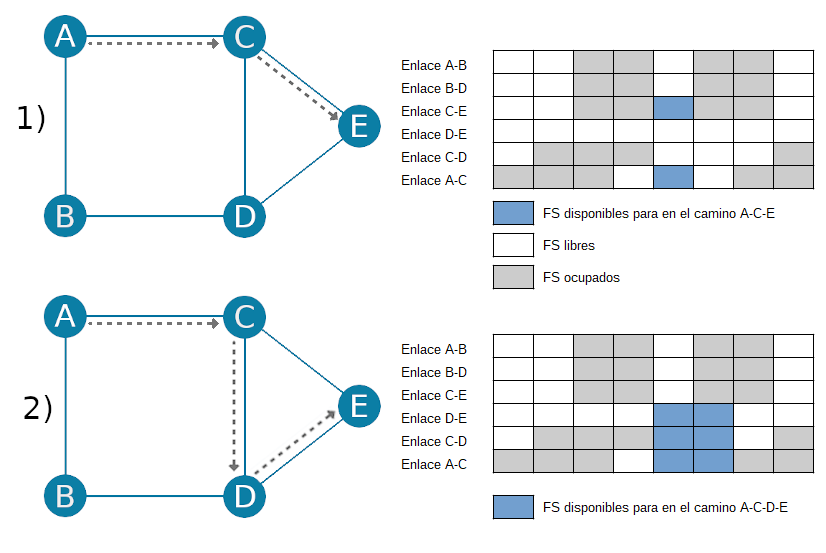
\includegraphics[width=1\textwidth]{capitulos/img/fragmentacion.png}
    \caption{Restricciones de contigüidad y continuidad en redes EON}
    \label{fig:fragmentacion}
\end{figure}

De esta manera es posible observar que quedan algunos bloques aislados, como los bloques de los enlaces A-C y sus enlaces adyacentes, en los cuales sus bloques difícilmente  sean utilizables ya que en su mayoría los bloques de un enlace no coinciden con el de los enlaces adyacentes. A esto es lo que llamamos fragmentación del espectro. 

\subsection{Enfoques de gestión de fragmentación}
El problema explicado anteriormente trae consigo efectos adversos para la red, provoca que la probabilidad de bloqueo de la red aumente, afectando directamente a su correcto y fluido funcionamiento. Debido a esto es importante encontrar mecanismos que ayuden a evitar, alivianar o disminuir la fragmentación del ancho de banda. 

Según la literatura científica existen diversos enfoques a ser considerados para la gestión de la desfragmentación , en la figura \ref{fig:gestion_fragmentacion} se muestran los principales enfoques de gestión de la fragmentación \cite{chatterjee2017fragmentation}.

\begin{figure}
    \centering
    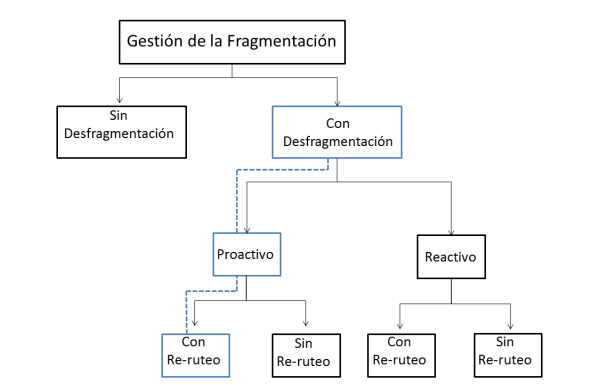
\includegraphics[width=1\textwidth]{capitulos/img/Gestion_Fragmentacion.PNG}
    \caption{Esquema de Gestión de la Fragmentación}
    \label{fig:gestion_fragmentacion}
\end{figure}

La Desfragmentación es un proceso en el cual se realiza la reconfiguración o re-ruteo de un sub-conjunto de conexiones existentes en la red, cuyo objetivo principal es reacomodar las asignaciones de espectro de las demandas de tráfico existentes
para consolidar los espacios disponibles en grandes bloques contiguos y continuos que pueden ser utilizados para establecer futuras demandas \cite{talebi2014spectrum}.

Es posible gestionar el problema de la fragmentación sin utilizar técnicas de desfragmentación del espectro (Sin Desfragmentación), esto se logra realizando una gestión del espectro con el objetivo de evitar su fragmentación.

En el tratamiento de la fragmentación siguiendo un esquema Sin Desfragmentación podemos mencionar a los algoritmos denominados Sensibles a la Fragmentación o \textit{Fragmentation Aware RSA} (FA-RSA). Los mismos consideran la fragmentación del ancho de banda para establecer las demandas siguiendo distintos indicadores de fragmentación y de esta manera se trata de minimizar la fragmentación del espectro.

Otra manera sería emplear técnicas de desfragmentación, utilizando dos enfoques principales:
\begin{itemize}
         \item Desfragmentación Reactiva: El proceso se realiza ante el bloqueo de una demanda, con el objetivo de conseguir su establecimiento.
         \item Desfragmentación Proactiva: Se realiza periódicamente o considerando ciertos valores que disparen el proceso, de esta forma se logra disminuir la fragmentación de la red y se minimiza la aparición de futuros bloqueos de demandas.
\end{itemize}
Los enfoques que utilizan técnicas de desfragmentación también pueden clasificarse en: (i) enfoques sin re-ruteo, que realizan sólo una reasignación del espectro en los \textit{lightpaths} o caminos de luz existentes, y (ii) con re-ruteos, que son técnicas que cambian las rutas y el espectro de los lightpaths existentes.

En el presente trabajo para la gestión de la fragmentación se utilizó el enfoque con desfragmentacion, proactiva y con re-ruteos de lightpaths existentes, en la figura \ref{fig:gestion_fragmentacion} se puede ver resaltado dicha estrategia.

\section{Descripción del problema tratado}
La Fragmentación del Ancho de Banda en Redes Ópticas Elásticas (EON) es un problema que afecta a la eficiencia en la utilización de recursos, el rendimiento de la red termina siendo profundamente afectada ya que este fenómeno podría provocar bloqueos de demandas por falta de ranuras disponibles contiguas y alineadas entre enlaces inmediatos y no necesariamente porque el espectro está totalmente ocupado. En secciones anteriores se explicaron estrategias para manejar la fragmentación de la red, en este trabajo se analiza la estrategia con desfragmentación, considerando un enfoque proactivo.

Un método ampliamente utilizado consiste en ejecutar el proceso de desfragmentación manera periódica con el fin de prevenir bloqueos futuros, abordando así una de las cuatro preguntas planteadas por Zhang \cite{zhang2014dynamic}, ¿Cuándo reconfigurar?.

En la figura \ref{fig:ejemploPeriodico} podemos ver una posible solución al problema de la selección del momento a realizar la desfragmentación, el cual consiste en realizar desfragmentaciones periódicas en tiempos fijos, en este caso cada 100 unidades de tiempo, el eje vertical indica el volumen de tráfico medido en el número de conexiones activas y el eje horizontal indica las unidades de tiempo, cada punto azul representa el momento en que el proceso de desfragmentación se ejecuta. Siguiendo este patrón se aprecia que se dan casos donde se realizan procesos de desfragmentación cuando la red podría no estar necesitando, si se considera que la utilización de la red es un indicador importante del grado de fragmentación. 

Además de la utilización de la red, se tienen otras métricas de fragmentación importantes, cuyos valores deben tenerse en cuenta para el disparo de los procesos de desfragmentación.

De esta forma vemos la necesidad de un disparador inteligente para ejecutar el proceso de desfragmentación que considere todos estos parámetros o ``características'' para seleccionar convenientemente el momento del disparo, ya que realizar muchas desfragmentaciones de manera frecuente afectan directamente al rendimiento de la red pudiendo causar disrupciones en las conexiones activas y en caso de realizar pocas y muy dispersas desfragmentaciones los efectos de las mismas serían casi imperceptibles.

En síntesis, la selección del momento para realizar el proceso de desfragmentación es crítica debido a que tiene un efecto importante en la cantidad de procesos de desfragmentación y esto tiene efecto en las dos métricas globales más importantes en el ruteo de redes elásticas las cuales son: Cantidad de bloqueos y Cantidad de reconfiguraciones. 

En los siguientes capítulos presentamos y abordamos en profundidad un modelo de disparo inteligente, que tiene en cuenta numerosos factores tales como métricas de fragmentación de la red, utilización de la red y bloqueos de demandas.
 
\begin{figure}[h!]
    \centering
    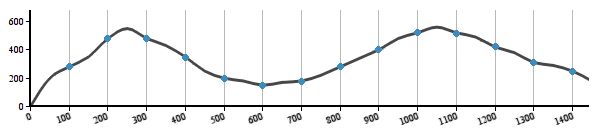
\includegraphics[width=1\textwidth]{capitulos/img/ejemploPeriodico.png}
    \caption{Ejemplo de desfragmentaciones periódicas con volumen de carga de tráfico variado}
    \label{fig:ejemploPeriodico}
\end{figure}



\section{Análisis Bibliográfico}     
%El trabajo presentado por M. Quagliotti \cite{quagliotti2017spectrum} propone un algoritmo RSA que busca mantener bajo el índice de fragmentación mediante el uso de una heurística básica durante la asignación del espectro, también brinda una amplia y útil descripción de métricas para evaluar la fragmentación del espectro.

%Para recopilar el conjunto de métricas de fragmentación utilizadas, realizaron un extenso estudio de la literatura científica, las cuales son: Utilization Entropy (UE), Shannon Entropy (SHF), External Fragmentation (EF), Access Blocking Probability (ABP), Compactness (SC) y High-slot Mark (HSM).

%Cada métrica de fragmentación proporciona su propia y peculiar medida de ocupación del espectro, relacionadas a la accesibilidad de recursos para el caso de EF, y ABP, grado de desorden y entropía en UE y SHF y compacidad del espectro ocupado en SC.

%Para nuestra investigación utilizamos algunas de las métricas presentadas en el mencionado articulo, las cuales nos sirven como características esenciales en la construcción de nuestro modelo de predicción de probabilidades de bloqueo.  

Seguidamente presentamos un análisis bibliográfico de trabajos presentes en el estado del arte que abordaron el mismo problema.

Jaume Comellas, Laura Vicario, y Gabriel Junyent \cite{comellas2018periodic} nos presentan un análisis de la desfragmentación periódica en redes EON con un tráfico dinámico, evaluando los diferentes efectos de los parámetros de desfragmentación en el rendimiento de la red.

El enfoque presentado en el trabajo consiste en realizar las desfragmentaciones en periodos fijos de N unidades de tiempo, con el principal objetivo de encontrar valores adecuados de N, ya que periodos de desfragmetación muy pequeños implican tener el espectro tan compactado como sea posible, pero a expensas de ejecutar el algoritmo con demasiada frecuencia, lo cual añade complejidad al proceso. Por otro lado, para valores muy altos de N, los efectos de la desfragmentación son insignificantes.

Este tipo de desfragmentaciones en periodos fijos es utilizado ampliamente en distintas investigaciones tales cómo \cite{davalos2019spectrum}, \cite{luo2012partial}, entre otros. En nuestra investigación utilizamos esta técnica a fin de comparar los resultados con el disparador que proponemos.

Otra manera de afrontar el enfoque proactivo del proceso de desfragmentación es realizarlo mediante algún tipo de disparador de tal manera que la misma sea ejecutada solo en periodos de tiempo donde es realmente necesaria, a continuación, veremos algunos artículos los cuales usaron esta estrategia.

La investigación realizada por Yutaka Takita y colegas \cite{takita2016wavelength} propone un mecanismo de disparo para el proceso de desfragmentación basado en el valor del \textit{High-slot Mark} (HM) el cual indica el número máximo de una ranura ocupada en la red. Utilizan esta métrica ya que lo consideran como una medida válida para evaluar la eficiencia en la utilización de los recursos. El proceso de desfragmentación se dispara de manera aleatoria cuando el valor del HM es mayor a un valor de \( HM_{max} \) definido previamente, en el artículo mencionado utilizan 30 como valor para \( HM_{max} \). 

Para el proceso de disparo en nuestro método propuesto se utilizan un conjunto de características o parámetros que indican el estado actual de la red, parte de ellas al igual que el \textit{High-slot Mark} son también métricas que indican la fragmentación del espectro. En el capitulo 4 se explican en profundidad estas características donde una de ellas es el llamado \textit{Maximum Slot Index} (MSI) el cual tiene una definición equivalente al del \textit{High-slot Mark}. 

Otra propuesta para el disparo es presentada por Ricardo V. Fávero y colegas \cite{favero2015new}. En su método combinan el enfoque reactivo y el enfoque proactivo para determinar el periodo en el que será ejecutado el proceso de desfragmentación, en la figura \ref{fig:favero} se puede observar el diagrama que ilustra el algoritmo propuesto.

Inicialmente la variable \textit{d} que utilizan para representar el estado de fragmentación se coloca en 0, el proceso de desfragmentación (DS) se ejecuta al cumplirse alguna de las siguientes condiciones.

Si se intenta establecer una demanda y no se encuentra un camino disponible para la misma, se verifica la variable \textit{d}, si esta se encuentra en 0 se ejecuta el proceso \textit{DS}, si no se logra establecer la demanda aun después del proceso de desfragmentación la misma se bloquea y la variable \textit{d} se cambia a 1.

La otra posibilidad de ejecución es cuando se intenta liberar una demanda, se ejecuta el proceso \textit{DS} sí \textit{d} = 1 y si la cantidad de \textit{lighpaths} liberados (\textit{r}) es igual a la variable predefinida previamente \textit{R}. 

Como se puede ver el método propuesto considera principalmente las conexiones liberadas por lo que puede considerarse como periódica.


\begin{figure}[h!]
    \centering
    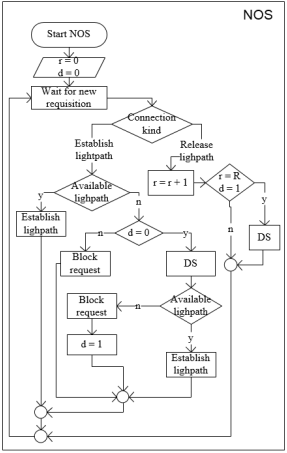
\includegraphics{capitulos/img/disparoFavero}
    \caption{Algoritmo propuesto por Favero y colegas \cite{favero2015new}}
    \label{fig:favero}
\end{figure}

Mingyang Zanhg y colegas plantean en su investigación \cite{zhang2013bandwidth} un disparo para el proceso de desfragmentación basado en la cantidad de conexiones liberadas. Básicamente consiste en ejecutar la desfragmentación cuándo la cantidad de conexiones liberadas es igual al parámetro fijo \textit{TH} (\textit{Threshold}). En su investigación utilizaron 300 como valor de \textit{TH}.

El trabajo presentado por Jie Zhang y colegas \cite{zhang2012priority}, proponen un disparo basado en el concepto de \textit{Spectrum Compacteness} o Compacidad del Espectro (SC) el cual es una métrica de fragmentación.

Para determinar el momento del disparo para el proceso de desfragmentación tienen en cuenta los siguientes pasos:  
\begin{enumerate}[label=\arabic*)]
    \item Seleccionar un valor apropiado de \textit{Spectrum Compactness} (SC) para actuar como umbral (T) para el disparo de la desfragmentación.
    \item Actualizar el valor de SC después de liberar conexiones o al establecer una nueva conexión. 
    \item Comparar los valores de SC y T; si SC < T disparar la desfragmentación y pasar al siguiente paso, sino volver al paso 2.
    \item Actualizar el ultimo valor de SC después de la desfragmentación y volver al paso 3.
\end{enumerate}

Por último el trabajo propuesto por Zhang y colegas \cite{zhang2014dynamic} presentan un análisis del problema de la desfragmentación de redes EON dividido en cuatro sub-problemas, el tercero de ellos es ¿Cuándo reconfigurar?.

Para el tercer subproblema plantean un algoritmo de disparo el cual tiene en cuenta la probabilidad de bloqueo instantánea (B) en un periodo \(\Delta \)t \((B(\Delta t))\) y la utilización del ancho de banda. 
De esta forma buscan realizan la comparación entre \(B(\Delta t)\) con \(B_{th}\) (umbral de probabilidad de bloqueo para el disparo del proceso de desfragmentación) solo cuando la red se encuentra con un crecimiento en la utilización del ancho de banda. 
\newpage

